\chapter{Applications of Private Blockchains in the Cosmos SDK}
\label{ch:private}

Private blockchains have emerged as an alternative to public blockchains, with a focus on privacy, control, and performance. Private blockchains are permissioned, meaning that access to the network is restricted to a select group of users, rather than being open to anyone. This offers several advantages, such as increased efficiency, scalability, and security. Private blockchains can also provide privacy and confidentiality, which is crucial for many applications that deal with sensitive data.

Private blockchains have a wide range of use cases, including supply chain management, identity management, voting systems, financial services, and more. The use cases of private blockchains are virtually unlimited, and new applications are being developed every day. With the increasing adoption of this technology, we can expect to see even more use cases emerge, as organizations look for new ways to leverage the benefits of blockchain technology.

Despite their many advantages, private blockchains also have some disadvantages. One of the main criticisms of private blockchains is that they are not truly decentralized, as the network is controlled by a select group of participants. This has led some to question whether private blockchains are truly blockchain technology or simply distributed databases. Additionally, the need for permissioned access can lead to slower adoption and reduced network effects, as organizations may be hesitant to join a closed network.

Overall, private blockchains offer a promising alternative to public blockchains, with unique advantages and use cases. As the technology continues to evolve and new applications emerge, we can expect to see even more innovative use cases and potential benefits.

\section{Designing Private Blockchains with Cosmos SDK}

In section \ref{ch:applicatoins-architecture} we introduced the concept of modules and how its high level abstraction allows developers to create custom blockchains. During this section we will dive deeper into technological aspects of the framework and what tools can be used to transform a specific use case into a distributed ledger.

When designing a private blockchain with the Cosmos SDK, the first step is to model your state and how it will change through messages\footnote{Transactions are referred as messages in the Cosmos SKD environment.}. This involves defining the data structures and functions that will be used to represent the state of the blockchain and the messages that will be used to update it.

By default, the main store of Cosmos SDK applications is a multistore, i.e. a store of stores. Developers can add any number of key-value stores to the multistore, depending on their application needs. The multistore exists to support the modularity of the Cosmos SDK, as it lets each module declare and manage their own subset of the state, as seen in Fig\ref{fig:application-multistore}. Key-value stores in the multistore can only be accessed with a specific capability key, which is typically held in the keeper of the module that declared the store.

\begin{figure}[H]
    \centering
    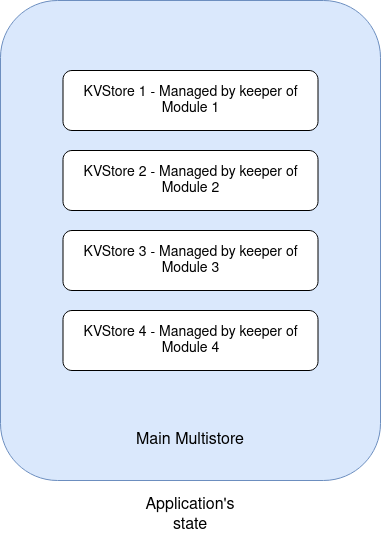
\includegraphics[scale=0.45]{figures/multistore.png}
    \caption{Application's state}
    \label{fig:application-multistore}
\end{figure}

Now that we have drawn the logic for storing information, we need to define how to modify it. Transactions are messages that contain instructions for updating the state of the blockchain. When a transaction is processed, it may modify the state of the blockchain by creating new data, updating existing data, or deleting data. For example, a transaction might transfer funds from one account to another, or it might create a new user account. When a transaction is submitted to the blockchain, it is validated by the consensus algorithm to ensure that it is valid and authorized by the appropriate parties. Once the transaction is validated, it is added to a block in the blockchain, and the state of the blockchain is updated to reflect the changes made by the transaction.

Queries, on the other hand, are messages that are used to retrieve information from the state of the blockchain. Queries do not modify the state of the blockchain, but instead return a read-only view of the data stored in the blockchain. Queries can be used to retrieve data such as account balances, transaction histories, or other metadata.

Nonetheless, the underlying core of the blockchain manages information directly in bytes. That means that transactions, queries and the state of the blockchain needs to be translated to raw bytes. Protobuf is a language-agnostic serialization tool that allows you to define a schema for your data, which can then be used to generate code in multiple programming languages. Protobuf is used extensively in the Cosmos SDK to define the structure of messages, transactions, and other data used in the blockchain allowing to marshall data into bytes and vice versa.

Last but not least, we need to access the functionalities of our blockchain application. The Cosmos SDK offers two main ways to do so, \gls{grpc} (REST api can be generated based on the gRPC endpoints) and the CLI interface. \gls{grpc} is a high-performance RPC framework that allows you to define services and methods that can be called remotely over a network\cite{gRPC-website}. With gRPC, you can define an API for your blockchain application, which can then be used to interact with the blockchain from other systems. gRPC uses Protobuf as its serialization format, which makes it fast, efficient, and easy to use.

Overall, the use of Protobuf and gRPC in the Cosmos SDK allows developers to create efficient and scalable blockchain applications that can be easily integrated with other systems. The combination of these two tools helps to make the development process more streamlined and efficient, while also improving the overall performance of the blockchain.

\section{Case Study: Private Blockchain for Crowdfunding}

In this section, we will provide a case study on how to build a private blockchain for crowdfunding using the Cosmos SDK. Crowdfunding is a way of raising funds from a large number of people, usually via the internet. Blockchain technology can bring several benefits to the world of crowdfunding by providing greater transparency, security, efficiency and confidence.

\notebox{
    For the sake of simplicity we won't modify the consensus engine for this case study and will stick with the default one. Although, you can technically customize the consensus engine which Cosmos uses it involves dealing with low level configurations surpassing the scope of this paper.
}

\subsection{Define Application State}

The first step in designing a blockchain application, such as a private blockchain for crowdfunding, is to understand the business needs and requirements of the application. Once we have a clear understanding of the information that needs to be stored in the blockchain, we can start modeling the state of the blockchain using a protobuf definition.

For our specific use case of crowdfunding, the information that needs to be stored in the blockchain includes details about the project, its sponsor, target funding, current funding, state, investors, and stages. We can use the protobuf definition shown in Listing~\ref{lst:project} to capture this information.

\begin{lstlisting}[language=go, caption=Project definition,label={lst:project}]

message Project {
  uint64                            id = 1;
  string                            sponsor = 2;
  cosmos.base.v1beta1.Coin          target = 3      [(gogoproto.nullable) = false];
  cosmos.base.v1beta1.Coin          current = 4     [(gogoproto.nullable) = false];
  string                            state = 5;
  repeated Investor                 investors = 6;
  repeated Stage                    stages = 7;
}

message Investor {
    string                           address  = 1;
    cosmos.base.v1beta1.Coin         equity   = 2 [(gogoproto.nullable) = false];
    int64                            profit   = 3;
}

message Stage {
    string                          name        = 1;
    cosmos.base.v1beta1.Coin        allocation  = 2 [(gogoproto.nullable) = false];
}
\end{lstlisting}

In the given protobuf definition, the \texttt{Project} message contains fields such as \texttt{id}, \texttt{sponsor}, \texttt{target}, \texttt{current}, \texttt{state}, \texttt{investors}, and \texttt{stages}. The \texttt{repeated} key word allows to create an array of the specified data type. In this case \texttt{Investor} and \texttt{Stage} are custom defined.

By using this protobuf definition, we can store all the necessary information regarding projects in the blockchain and ensure that it is structured and accessible. Transactions and queries can then be built on top of this state to allow investors to contribute to the project, track their equity, and receive their share of the profits.

\subsection{Modify the State of the Application}

To modify the projects stored in the blockchain, we need to create transactions that encapsulate the desired modifications. This involves defining the protobuf message for the transaction, the \gls{cli} interface definition and implementing the corresponding message server to interact with the keeper.

To interact with the message server and modify the state of the application, we have multiple options available. One option is to use the \gls{grpc} endpoints as defined in Lst~\ref{lst:gRPC-endpoint}, which allows for remote procedure calls to be made to the message server. With the gRPC endpoints, clients can send requests to modify projects over the network, enabling seamless integration with external systems or user interfaces.

Another option is to use the CLI provided by the Cosmos SDK. The CLI provides a convenient command-line interface for interacting with the blockchain and executing transactions. By using the appropriate commands and providing the necessary transaction details, the CLI can be used to modify the state of the application directly.

\begin{lstlisting}[language=go, caption=gRPC endpoints definition,label={lst:gRPC-endpoint}]
service Msg {
  rpc CreateProject(MsgCreateProject) returns (MsgCreateProjectResponse);
  rpc InvestorBuyIn(MsgInvestorBuyIn) returns (MsgInvestorBuyInResponse);
  rpc ChangeState(MsgChangeState) returns (MsgChangeStateResponse);
  rpc MoneyIn(MsgMoneyIn) returns (MsgMoneyInResponse);
  rpc MoneyOut(MsgMoneyOut) returns (MsgMoneyOutResponse);
  rpc SponsorCancel(MsgSponsorCancel) returns (MsgSponsorCancelResponse);
  rpc SponsorAccept(MsgSponsorAccept) returns (MsgSponsorAcceptResponse);
  rpc AdminAdd(MsgAdminAdd) returns (MsgAdminAddResponse);
  rpc AdminDelete(MsgAdminDelete) returns (MsgAdminDeleteResponse);
  rpc NextStage(MsgNextStage) returns (MsgNextStageResponse);
  rpc ShareProfit(MsgShareProfit) returns (MsgShareProfitResponse);
  rpc UpdateDraftProject(MsgUpdateDraftProject) returns (MsgUpdateDraftProjectResponse);
}
\end{lstlisting}

\subsection{Query the State of the Application}

In addition to modifying the state of the blockchain, it is often necessary to query the state to retrieve specific information from the blockchain. This allows users and applications to access project details, investor information, and other relevant data stored in the blockchain.

To query the state of the application, we need to define protobuf messages that represent the query requests and responses. These messages specify the data we want to retrieve and the format in which the data should be returned. Lst~\ref{lst:query-proto} shows and example of the query definition to retrieve a list of all the projects.

Once we have defined the protobuf messages, we can implement query handlers to handle the query requests. Query handlers receive the query requests, interact with the keeper to retrieve the requested data, and construct the corresponding query responses.

Similar to modifying the state, querying the state of the application can be done through the \gls{grpc} endpoint or the CLI interface. With the gRPC endpoint, clients can send query requests to the message server, which in turn interacts with the keeper to retrieve the requested information. The gRPC endpoint allows for efficient and structured retrieval of data, making it suitable for integration with external systems or user interfaces. Alternatively, the CLI interface provides a command-line interface for executing queries directly.

\begin{lstlisting}[language=go, caption=Query gRPC Definition,label={lst:query-proto}]
service Query {
    rpc Params (QueryParamsRequest) returns (QueryParamsResponse) {
        option (google.api.http).get = "/therealblock/params";
      }
      rpc ListProjects (QueryListProjectsRequest) returns (QueryListProjectsResponse) {
        option (google.api.http).get = "/therealblock/list_projects";
      } 
      rpc GetProject (QueryGetProjectRequest) returns (QueryGetProjectResponse) {
        option (google.api.http).get = "/therealblock/get_project/{id}";
      }
      rpc ListAdmins (QueryListAdminsRequest) returns (QueryListAdminsResponse) {
        option (google.api.http).get = "/therealblock/list_admins";
      }
      rpc GetProjectStage (QueryGetProjectStageRequest) returns (QueryGetProjectStageResponse) {
        option (google.api.http).get = "/therealblock/project_stage/{projectId}";
      }
}
\end{lstlisting}

\subsection{Project Set Up}

To enable projects creation on the crowdfunding platform, we use the transaction message \texttt{CreateProject} defined in the protobuf definition Lst~\ref{lst:gRPC-endpoint}. This message contains all the necessary information required to create a new project, such as the sponsor's name, target funding amount, and the stages of the project. The \texttt{CreateProject} message handler, processes the incoming transaction and updates the blockchain's state accordingly.

\begin{lstlisting}[language=go, caption=CreateProject protobuf definition,label={lst:create_project_proto}]
message MsgCreateProject {
  string                 sponsor = 1;
  cosmos.base.v1beta1.Coin target  = 2 [(gogoproto.nullable) = false];
  repeated Stage         stages  = 3;
}
\end{lstlisting}

\begin{lstlisting}[language=go, caption=CreateProject CLI protobuf definition,label={lst:create-project-cli}]
func CmdCreateProject() *cobra.Command {
	cmd := &cobra.Command{
		Use:   "create-project [target] [stages]",
		Short: "Broadcast message create-project",
		Args:  cobra.ExactArgs(2),
		RunE: func(cmd *cobra.Command, args []string) (err error) {
			argTarget, err := sdk.ParseCoinNormalized(args[0])
			if err != nil {
				return err
			}
			argStages, err := types.ParseStageNormalized(args[1])
			if err != nil {
				return err
			}
			clientCtx, err := client.GetClientTxContext(cmd)
			if err != nil {
				return err
			}
			msg := types.NewMsgCreateProject(
				clientCtx.GetFromAddress().String(),
				argTarget,
				argStages,
			)
			if err := msg.ValidateBasic(); err != nil {
				return err
			}
			return tx.GenerateOrBroadcastTxCLI(clientCtx, cmd.Flags(), msg)
		},
	}
	flags.AddTxFlagsToCmd(cmd)
	return cmd
}
\end{lstlisting}

When a user wants to create a project, they initiate a transaction by using the \gls{cli} command, defined in Lst~\ref{lst:create-project-cli},  or by making a gRPC request to the message server. For instance, using the Cosmos SDK \gls{cli}, the command to create a project would look like:

\begin{verbatim}
$ daemonNamed tx appName create-project --sponsor "Project Sponsor" \
    --target "1000TOKENNAME" \
    --stages "Stage 1:100TOKENNAME,Stage 2:500TOKENNAME"
\end{verbatim}

The command above will generate a transaction containing the \texttt{CreateProject} message with the specified details, and upon successful inclusion in a block, a new project will be created with the given information.

In the backend, the message server will receive the gRPC request with the \texttt{CreateProject} message, and the corresponding message handler will be invoked. The handler will validate the transaction and check if the sponsor address is authorized to create projects. The keeper method to add authorized addresses is shown in Lst~\ref{lst:add-admin}. If all checks pass, a new project instance will be created, and its details will be stored in the application's state, Lst~\ref{lst:keeper_create_project}.

\newpage

\begin{lstlisting}[language=go, caption=Keeper implementation for CreateProject,label={lst:keeper_create_project}]
func (k msgServer) CreateProject(goCtx context.Context, msg *types.MsgCreateProject) (*types.MsgCreateProjectResponse, error) {
	ctx := sdk.UnwrapSDKContext(goCtx)
	var project = types.Project{
		Stages:  msg.Stages,
		Sponsor: msg.Sponsor,
		Target:  msg.Target,
	}
	id, err := k.AppendProject(
		ctx,
		project,
	)
	if err != nil {
		return &types.MsgCreateProjectResponse{}, err
	}
	types.EmitEvent(ctx, types.EventTypeProjectCreated, id, msg.Sponsor)
	return &types.MsgCreateProjectResponse{
		Id:      id,
		Address: msg.Sponsor,
	}, nil
}
\end{lstlisting}

\begin{lstlisting}[language=go, caption=Keeper implementation for CreateProject,label={lst:add-admin}]
func (k msgServer) AdminAdd(goCtx context.Context, msg *types.MsgAdminAdd) (*types.MsgAdminAddResponse, error) {
	ctx := sdk.UnwrapSDKContext(goCtx)
	if !k.IsAdminAccount(ctx, msg.Creator) {
		return nil, types.ErrNotAdminAccount
	}
	if k.IsAdminAccount(ctx, msg.NewAddress) {
		return nil, types.ErrAdminAccountExists
	}
	k.setAdminAccount(ctx, types.Account{Address: msg.NewAddress})
	if !k.IsAdminAccount(ctx, msg.NewAddress) {
		return nil, types.ErrAdminAccountNotSet
	}
	return &types.MsgAdminAddResponse{
		Address: msg.NewAddress,
	}, nil
}
\end{lstlisting}

With the \texttt{CreateProject} transaction successfully processed, projects can be added to the blockchain's state.

\subsection{Updating Draft Projects}

When a project is first created, it's in \texttt{draft} state, meaning its details are subject to change and refinement. To update a project's information, authorized users can perform the \texttt{UpdateDraftProject} transaction. This transaction message allows to modify specific details of the project, such as the target, funding or stages of the project.

\begin{lstlisting}[language=go, caption=UpdateDraftProject protobuf definition,label={lst:update_draft_project_proto}]
message MsgUpdateDraftProject {
  string                                creator   = 1;
  uint64                                projectId = 2;
  cosmos.base.v1beta1.Coin              target    = 4 [(gogoproto.nullable) = false];
  repeated Stage                        stages    = 5;
}
\end{lstlisting}

To execute the \texttt{UpdateDraftProject} transaction, the user must be authorized to modify the project. The message handler, Lst~\ref{lst:keeper-update-draft}, will perform the necessary checks to ensure the user has the proper authorization and then proceed to update the project with the new information.

\newpage
\begin{lstlisting}[language=go, caption=Keeper implementation for UpdateDraftProject ,label={lst:keeper-update-draft}]
func (k msgServer) UpdateDraftProject(goCtx context.Context, msg *types.MsgUpdateDraftProject) (*types.MsgUpdateDraftProjectResponse, error) {
	ctx := sdk.UnwrapSDKContext(goCtx)
	projectId, err := k.updateDraftProjectInfo(ctx, msg.ProjectId, msg.Target, msg.Stages, msg.Creator)
	if err != nil {
		return nil, err
	}
	return &types.MsgUpdateDraftProjectResponse{
		ProjectId: projectId,
	}, nil
}
func (k Keeper) updateDraftProjectInfo(ctx sdk.Context, projectId uint64, target sdk.Coin, stages []*types.Stage, signer string) (uint64, error) {
	project, found := k.getProjectId(ctx, projectId)
	if !found {
		return 0, types.ErrProjectNotFound
	}
	if strings.Compare(signer, project.Sponsor) != 0 {
		return 0, types.ErrNotProjectSponsor
	}
	if strings.Compare(project.State, types.ProjectStateDraft) != 0 {
		return 0, types.ErrProjectNotDraft
	}
	if err := k.checkStages(stages, target); err != nil {
		return 0, err
	}
	project.Target = target
	project.Stages = stages
	k.saveProject(ctx, &project)
	return project.Id, nil
}
\end{lstlisting}

The \texttt{UpdateDraftProject} transaction provides flexibility during the early stages of a project when its details may evolve based on feedback or changing requirements. However, once the project details are finalized, it is time to promote the project to the \texttt{active} state, enabling investors to participate.

\begin{lstlisting}[language=go, caption=Create Project CLI  definition,label={lst:update-draft-cli}]
func CmdUpdateDraftProject() *cobra.Command {
	cmd := &cobra.Command{
		Use:   "update-draft-project [project-id] [target] [stages]",
		Short: "Broadcast message update-draft-project",
		Args:  cobra.ExactArgs(3),
		RunE: func(cmd *cobra.Command, args []string) (err error) {
			argProjectId, err := cast.ToUint64E(args[0])
			if err != nil {
				return err
			}
			argTarget, err := sdk.ParseCoinNormalized(args[1])
			if err != nil {
				return err
			}
			argStages, err := types.ParseStageNormalized(args[2])
			if err != nil {
				return err
			}
			clientCtx, err := client.GetClientTxContext(cmd)
			if err != nil {
				return err
			}
			msg := types.NewMsgUpdateDraftProject(
				clientCtx.GetFromAddress().String(),
				argProjectId,
				argTarget,
				argStages,
			)
			if err := msg.ValidateBasic(); err != nil {
				return err
			}
			return tx.GenerateOrBroadcastTxCLI(clientCtx, cmd.Flags(), msg)
		},
	}
	flags.AddTxFlagsToCmd(cmd)
	return cmd
}
\end{lstlisting}

The transaction can be initiated by using the \gls{cli} command, defined in Lst~\ref{lst:update-draft-cli},  or by making a \gls{grpc} request to the message server. For instance, using the Cosmos SDK CLI, the command to create a project would look like:


\begin{verbatim}
$ daemonNamed tx appName update-draft-project --project-id "idNumber" \
    --target "1000TOKENNAME" \
    --stages "Stage 1:100TOKENNAME,Stage 2:500TOKENNAME"
\end{verbatim}

\subsection{Project Activation}

The transition from the `draft` stage to the `active` stage marks the activation of a project on the private blockchain for crowdfunding. During the `active` stage, the project becomes open for investment, allowing investors to participate and contribute funds.

\begin{lstlisting}[language=go, caption=ChangeState protobuf definition,label={lst:change-state-proto}]
message MsgChangeState {
  string creator   = 1;
  uint64 projectId = 2;
  string newState  = 3;
}
\end{lstlisting}

To activate a project, sponsors utilize the `ChangeState` transaction with the appropriate parameters, Lst~\ref{lst:change-state-proto}. The message handler, Lst~\ref{lst:keeper-change-state}, will ensure the user has the proper authorization and then proceed to update the blockchain state.

\begin{lstlisting}[language=go, caption=Keeper implementation for ChangeState ,label={lst:keeper-change-state}]
func (k msgServer) ChangeState(goCtx context.Context, msg *types.MsgChangeState) (*types.MsgChangeStateResponse, error) {
	ctx := sdk.UnwrapSDKContext(goCtx)
	if !k.IsAdminAccount(ctx, msg.Creator) {
		return nil, types.ErrNotAdminAccount
	}
	projectId, err := k.changeProjectState(ctx, msg.NewState, msg.ProjectId)
	if err != nil {
		return &types.MsgChangeStateResponse{}, err
	}
	return &types.MsgChangeStateResponse{
		ProjectId: projectId,
	}, nil
}
\end{lstlisting}

\begin{lstlisting}[language=go, caption=Change State CLI Definition,label={lst:change-state}]
func CmdChangeState() *cobra.Command {
	cmd := &cobra.Command{
		Use:   "change-state [project-id] [new-state]",
		Short: "Broadcast message change-state",
		Args:  cobra.ExactArgs(2),
		RunE: func(cmd *cobra.Command, args []string) (err error) {
			argProjectId, err := cast.ToUint64E(args[0])
			if err != nil {
				return err
			}
			argNewState := args[1]
			clientCtx, err := client.GetClientTxContext(cmd)
			if err != nil {
				return err
			}
			msg := types.NewMsgChangeState(
				clientCtx.GetFromAddress().String(),
				argProjectId,
				argNewState,
			)
			if err := msg.ValidateBasic(); err != nil {
				return err
			}
			return tx.GenerateOrBroadcastTxCLI(clientCtx, cmd.Flags(), msg)
		},
	}
	flags.AddTxFlagsToCmd(cmd)
	return cmd
}
\end{lstlisting}

The sponsor initiates the transaction using the \gls{cli} command, implemented in Lst~\ref{lst:change-state}, or \gls{grpc} request, providing the project ID and setting the desired state as `active`. The command would look like this:

\begin{verbatim}
$ daemonNamed tx appName change-state --project-id "idNumber" \
    --state "active"
\end{verbatim}

\subsubsection{Investors Buy-In}
Once a project is in the `active` stage, investors can participate by utilizing the `InvestorBuyIn` transaction, Lst~\ref{lst:buy-in-proto} shows the message definition. The transaction allows investors to contribute funds to the project, becoming stakeholders in the crowdfunding initiative.

The message handler, Lst~\ref{lst:keeper-buy-in}, will allocate the investment made to the module which will act as a scrow agent until the project reaches the target amount. In which case, the project will move to `Funded` and the money will be released to the sponsor of the project. Meanwhile the investors will receive a wrapped token representing their initial investment in the project.

\newpage
\begin{lstlisting}[language=go, caption=InvestorbuyIn protobuf definition,label={lst:buy-in-proto}]
message MsgInvestorBuyIn {
  string                   investor  = 1;
  uint64                   projectId = 2;
  cosmos.base.v1beta1.Coin amount    = 3 [(gogoproto.nullable) = false];
}
\end{lstlisting}

\begin{lstlisting}[language=go, caption=Keeper implementation for Investor Buy-in ,label={lst:keeper-buy-in}]
func (k msgServer) InvestorBuyIn(goCtx context.Context, msg *types.MsgInvestorBuyIn) (*types.MsgInvestorBuyInResponse, error) {
	ctx := sdk.UnwrapSDKContext(goCtx)
	var investor = types.Investor{
		Address: msg.Investor,
		Equity:  msg.Amount,
	}
	appendedAddr, err := k.AppendInvestorBuyIn(ctx, msg.ProjectId, investor)
	if err != nil {
		return &types.MsgInvestorBuyInResponse{}, err
	}
	return &types.MsgInvestorBuyInResponse{
		InvestorAddr: appendedAddr,
	}, nil
}

func (k Keeper) AppendInvestorBuyIn(ctx sdk.Context, id uint64, investor types.Investor) (string, error) {
	if investor.Equity.Amount.Equal(sdk.ZeroInt()) {
		return "", types.ErrCoinZeroAmount
	}
	project, found := k.getProjectId(ctx, id)
	if !found {
		return "", types.ErrProjectNotFound
	}
	if project.State != types.ProjectStateActive {
		return "", types.ErrProjectNotActive
	}
	if strings.Compare(project.Target.Denom, investor.Equity.Denom) != 0 {
		return "", types.ErrCoinDiffDenom
	}
	if project.Target.Sub(project.Current).IsLT(investor.Equity) {
		return "", types.ErrOverFunded
	}
	addr, err := sdk.AccAddressFromBech32(investor.Address)
	if err != nil {
		return "", err
	}
	if err := k.bankKeeper.SendCoinsFromAccountToModule(ctx, addr, types.ModuleName, sdk.NewCoins(investor.Equity)); err != nil {
		return "", err
	}
	project.Investors = appendInvestor(project.Investors, &investor)
	project.Current = project.Current.Add(investor.Equity)
	if project.Target.IsEqual(project.Current) {
		project.State = types.ProjectStatePending
		types.EmitEvent(ctx, types.EventTypeProjectPending, project.Id, investor.Address)
	} else {
		types.EmitEvent(ctx, types.EventTypeProjectInvested, project.Id, investor.Address)
	}
	k.saveProject(ctx, &project)
	return investor.Address, nil
}
\end{lstlisting}
\newpage
\begin{lstlisting}[language=go, caption=Investor Buy-in CLI Definition,label={lst:investor-buy-in-cli}]
func CmdInvestorBuyIn() *cobra.Command {
	cmd := &cobra.Command{
		Use:   "investor-buy-in [project-id] [amount]",
		Short: "Broadcast message investor-buy-in",
		Args:  cobra.ExactArgs(2),
		RunE: func(cmd *cobra.Command, args []string) (err error) {
			argProjectId, err := cast.ToUint64E(args[0])
			if err != nil {
				return err
			}
			argAmount, err := sdk.ParseCoinNormalized(args[1])
			if err != nil {
				return err
			}
			clientCtx, err := client.GetClientTxContext(cmd)
			if err != nil {
				return err
			}
			msg := types.NewMsgInvestorBuyIn(
				clientCtx.GetFromAddress().String(),
				argProjectId,
				argAmount,
			)
			if err := msg.ValidateBasic(); err != nil {
				return err
			}
			return tx.GenerateOrBroadcastTxCLI(clientCtx, cmd.Flags(), msg)
		},
	}
	flags.AddTxFlagsToCmd(cmd)
	return cmd
}
\end{lstlisting}

Investors can execute the `InvestorBuyIn` transaction through the \gls{cli} command, implemented in Lst~\ref{lst:investor-buy-in-cli}, or \gls{grpc} request specifying the project ID and the amount they wish to invest. The command would look like this:

\begin{verbatim}
$ daemonNamed tx appName change-state --project-id "idNumber" \
    --investment-amount "1000TOKENNAEM"
\end{verbatim}

\subsection{Accept Project Funding}
\label{subsec:sponsor_accepts}

The `SponsorAccept` transaction is a crucial step in the crowdfunding process, allowing sponsors to accept project funding once the project has reached its funding target. 

The transaction message is defined in Lst~\ref{lst:sponsor_accepts_proto}. This transaction will allow to promote the project from `Pending` state, which is obtained when the project has meet the funding target, to `Funded` state. Allowing authorized accounts to either cancel or validate the project before starting it's development.

\begin{lstlisting}[language=go, caption=SponsorAccepts protobuf definition,label={lst:sponsor_accepts_proto}]
message MsgSponsorAccept {
  string creator   = 1;
  uint64 projectId = 2;
}
\end{lstlisting}

The message handler, Lst~\ref{lst:keeper-accept}, verifies that the transaction initiator is the authorized sponsor of the project in the `pending` state, awaiting acceptance. Once all conditions are met, the transaction is executed, and the project's state is updated to `funded`. This update triggers the release of the funds collected during the `active` stage to the sponsor's account (only the allocated fund to the first stage in the project's roadmap). Additionally, synthetic/wrapped tokens representing investors' contributions are minted and distributed among the investors, accurately representing their share in the project.

\newpage
\begin{lstlisting}[language=go, caption=Keeper implementation for SponsorAccept ,label={lst:keeper-accept}]
func (k msgServer) SponsorAccept(goCtx context.Context, msg *types.MsgSponsorAccept) (*types.MsgSponsorAcceptResponse, error) {
	ctx := sdk.UnwrapSDKContext(goCtx)
	projectId, err := k.sponsorAcceptProject(ctx, msg.ProjectId, msg.Creator)
	if err != nil {
		return nil, err
	}
	return &types.MsgSponsorAcceptResponse{
		ProjectId: projectId,
	}, nil
}
func (k Keeper) sponsorAcceptProject(ctx sdk.Context, projectId uint64, sponsor string) (uint64, error) {
	project, found := k.getProjectId(ctx, projectId)
	if !found {
		return 0, types.ErrProjectNotFound
	}
	if strings.Compare(project.Sponsor, sponsor) != 0 {
		return 0, types.ErrNotProjectSponsor
	}
	if project.State != types.ProjectStatePending {
		return 0, types.ErrProjectNotPending
	}
	project.State = types.ProjectStateFunded
	if err := k.issueProjectTokens(ctx, &project); err != nil {
		return 0, err
	}
	k.saveProject(ctx, &project)
	return project.Id, nil
}
\end{lstlisting}

The transaction can broadcasted using the \gls{cli} or \gls{grpc} request. The CLI command would look like this:

\begin{verbatim}
$ daemonNamed tx appName sponsor-accept --project-id "idNumber"
\end{verbatim}

\subsection{Advancing Projects through Stages}

The `NextStage` transaction is a pivotal component in the life cycle of a funded project within our crowdfunding application. This transaction empowers administrators to advance the project through its defined stages as milestones are met or mitigating the risk of failed/malicious projects, hence protecting investors' money.

The `NextStage` transaction is initiated by administrators to progress the project from the `funded` state to the next stage in its life cycle. Before executing the transaction, the business logic ensures the following conditions:

\begin{enumerate}
  \item Authorization: The initiator of the `NextStage` transaction must be an authorized administrator capable of advancing the project stages.
  \item Project State: The project must be in the `funded` state to proceed to the next stage. If the project is not in the `funded` state, the transaction cannot be executed.
  \item Calculate Next Stage: The business logic calculates the allocation required for the next stage and updates the project's state accordingly.
  \item Transfer of Funds: If the project has subsequent stages, the required allocation for the next stage is transferred from the project's current funding to the sponsor's account using the Cosmos SDK's `SendCoinsFromModuleToAccount` method.
  \item Project Completion: If the project has no more stages after the current one, the project's state is updated to `completed`.
\end{enumerate}

The `NextStage` transaction message is defined Lst~\ref{lst:next_stage_proto}. This message contains the project ID, which helps identify the specific project to advance to the next stage.

\newpage
\begin{lstlisting}[language=go, caption=NextStage protobuf definition,label={lst:next_stage_proto}]
message MsgNextStage {
  string creator   = 1;
  uint64 projectId = 2;
}
\end{lstlisting}

The `NextStage` transaction message is processed in the application's message handler, Lst~\ref{lst:next_stage_handler}. The handler verifies that the initiator of the transaction is an authorized administrator capable of advancing the project stages. It then calls the `nextProjectStage` function, which calculates the required allocation for the next stage and updates the project's state accordingly.

\begin{lstlisting}[language=go, caption=Keeper implementation for NextStage,label={lst:next_stage_handler}]
func (k msgServer) NextStage(goCtx context.Context, msg *types.MsgNextStage) (*types.MsgNextStageResponse, error) {
  ctx := sdk.UnwrapSDKContext(goCtx)
  if !k.IsAdminAccount(ctx, msg.Creator) {
    return nil, types.ErrNotAdminAccount
  }
  projectId, err := k.nextProjectStage(ctx, msg.ProjectId)
  if err != nil {
    return nil, err
  }
  return &types.MsgNextStageResponse{
    ProjectId: projectId,
  }, nil
}
func (k Keeper) nextProjectStage(ctx sdk.Context, projectId uint64) (uint64, error) {
	project, found := k.getProjectId(ctx, projectId)
	if !found {
		return 0, types.ErrProjectNotFound
	}
	if project.State != types.ProjectStateFunded {
		return 0, types.ErrProjectNotFunded
	}
	allocation, hasNext := calculateNextStage(project)
	if hasNext {
		sponsor, err := sdk.AccAddressFromBech32(project.Sponsor)
		if err != nil {
			return 0, err
		}
		if err := k.bankKeeper.SendCoinsFromModuleToAccount(ctx, types.ModuleName, sponsor, sdk.NewCoins(allocation)); err != nil {
			return 0, err
		}
		project.Current = project.Current.Sub(allocation)
	} else {
		project.State = types.ProjectStateCompleted
	}
	k.saveProject(ctx, &project)
	return project.Id, nil
}
\end{lstlisting}

\begin{lstlisting}[language=go, caption=Next Stage CLI Definition,label={lst:next-cli}]
func CmdNextStage() *cobra.Command {
	cmd := &cobra.Command{
		Use:   "next-stage [project-id]",
		Short: "Broadcast message next-stage",
		Args:  cobra.ExactArgs(1),
		RunE: func(cmd *cobra.Command, args []string) (err error) {
			argProjectId, err := cast.ToUint64E(args[0])
			if err != nil {
				return err
			}
			clientCtx, err := client.GetClientTxContext(cmd)
			if err != nil {
				return err
			}
			msg := types.NewMsgNextStage(
				clientCtx.GetFromAddress().String(),
				argProjectId,
			)
			if err := msg.ValidateBasic(); err != nil {
				return err
			}
			return tx.GenerateOrBroadcastTxCLI(clientCtx, cmd.Flags(), msg)
		},
	}
	flags.AddTxFlagsToCmd(cmd)
	return cmd
}
\end{lstlisting}

Authorized administrators can broadcast the `NextStage` transaction using the \gls{cli}, implementatin showed in Lst~\ref{lst:next-cli} or \gls{grpc} request. The CLI command would look like this:

\begin{verbatim}
$ daemonNamed tx appName next-stage --project-id "idNumber"
\end{verbatim}

By utilizing the `NextStage` transaction, administrators play a crucial role in the progression of funded projects. The transaction ensures that projects move through their predefined stages as milestones are met, leading to efficient management and completion of crowdfunding initiatives.

\subsection{Distributing Profits to Shareholders}

The `ShareProfit` transaction is a critical step in the life cycle of a successful project within the private blockchain for crowdfunding. This transaction enables project sponsors to distribute profits to the shareholders when the project starts generating income.

The transaction message is defined in Lst~\ref{lst:share_profit_proto}. This message contains the project ID, the profit amount, and the address of the sponsor who initiated the transaction.

\newpage
\begin{lstlisting}[language=go, caption=ShareProfit protobuf definition,label={lst:share_profit_proto}]
message MsgShareProfit {
  string       creator   = 1;
  uint64       project_id = 2;
  cosmos.base.v1beta1.Coin amount    = 3 [(gogoproto.nullable) = false];
}
\end{lstlisting}

The `ShareProfit` transaction message is processed in the application's message handler Lst~\ref{lst:share_profit_handler}. The handler validates the initiator of the transaction, checks the project's existence, and ensures that the project sponsor initiates the transaction. Afterward, the profit is distributed among the project's shareholders based on their equity in the project.

\begin{lstlisting}[language=go, caption=Keeper implementation for ShareProfit,label={lst:share_profit_handler}]
func (k msgServer) ShareProfit(goCtx context.Context, msg *types.MsgShareProfit) (*types.MsgShareProfitResponse, error) {
  ctx := sdk.UnwrapSDKContext(goCtx)
  if strings.Compare(msg.Amount.Denom, "rbs") != 0 {
    return nil, types.ErrInvalidDenom
  }
  projectId, err := k.shareProfit(ctx, msg.ProjectId, msg.Amount, msg.Creator)
  if err != nil {
    return nil, err
  }
  return &types.MsgShareProfitResponse{
    ProjectId: projectId,
  }, nil
}
func (k Keeper) shareProfit(ctx sdk.Context, projectId uint64, profit sdk.Coin, signer string) (uint64, error) {
	project, found := k.getProjectId(ctx, projectId)
	if !found {
		return 0, types.ErrProjectNotFound
	}
	if strings.Compare(project.Sponsor, signer) != 0 {
		return 0, types.ErrNotProjectSponsor
	}
	if len(project.Investors) == 0 {
		return 0, types.ErrNoInvestors
	}
	sponsor, err := sdk.AccAddressFromBech32(project.Sponsor)
	if err != nil {
		return 0, err
	}
	if err := k.bankKeeper.SendCoinsFromAccountToModule(ctx, sponsor, types.ModuleName, sdk.NewCoins(profit)); err != nil {
		return 0, err
	}
	for _, investor := range project.Investors {
		addr, err := sdk.AccAddressFromBech32(investor.Address)
		if err != nil {
			return 0, err
		}
		var equity = profit.Amount.Mul(
			investor.Equity.Amount.Mul(sdkmath.NewInt(100)).Quo(
				project.Target.Amount)).Quo(
			sdkmath.NewInt(100))
		if err := k.bankKeeper.SendCoinsFromModuleToAccount(ctx, types.ModuleName, addr, sdk.NewCoins(sdk.NewCoin("rbs", equity))); err != nil {
			return 0, err
		}
		investor.Profit += equity.Int64()
	}
	k.saveProject(ctx, &project)
	return project.Id, nil
}
\end{lstlisting}

\begin{lstlisting}[language=go, caption=Share Profits CLI Definition,label={lst:share-cli}]
func CmdShareProfit() *cobra.Command {
	cmd := &cobra.Command{
		Use:   "share-profit [project-id] [amount]",
		Short: "Broadcast message share-profit",
		Args:  cobra.ExactArgs(2),
		RunE: func(cmd *cobra.Command, args []string) (err error) {
			argProjectId, err := cast.ToUint64E(args[0])
			if err != nil {
				return err
			}
			argAmount, err := sdk.ParseCoinNormalized(args[1])
			if err != nil {
				return err
			}
			clientCtx, err := client.GetClientTxContext(cmd)
			if err != nil {
				return err
			}
			msg := types.NewMsgShareProfit(
				clientCtx.GetFromAddress().String(),
				argProjectId,
				argAmount,
			)
			if err := msg.ValidateBasic(); err != nil {
				return err
			}
			return tx.GenerateOrBroadcastTxCLI(clientCtx, cmd.Flags(), msg)
		},
	}
	flags.AddTxFlagsToCmd(cmd)
	return cmd
}
\end{lstlisting}

Project sponsors can broadcast the `ShareProfit` transaction using the \gls{cli}, Lst~\ref{lst:share-cli} or \gls{grpc} request. The CLI command would look like this:

\begin{verbatim}
$ daemonNamed tx appName share-profit --project-id "idNumber" \
    --amount "1000TOKENNAEM"
\end{verbatim}

By utilizing the `ShareProfit` transaction, sponsors can ensure the fair distribution of profits to project shareholders, accurately reflecting each shareholder's equity in the project. This transaction reinforces transparency and trust within the private blockchain for crowdfunding.

\subsection{Wrapping Up}

In conclusion, messages and queries serve as fundamental components of blockchain applications, enabling seamless interaction with and retrieval of data from the blockchain. Understanding the business logic of the application is crucial for effectively modeling messages and queries, and the steps outlined in this section provide a structured approach to achieve this.

By understanding the specific requirements and objectives of the application, developers can model messages that encapsulate the necessary modifications to the blockchain state. Through the definition of protobuf messages and the implementation of message servers, the logic and modules of the application can be efficiently built. The flexibility of the Cosmos SDK allows for the adoption of various interaction options, such as the gRPC endpoint or the CLI interface, enhancing the usability and accessibility of the blockchain application.

Similarly, queries play a vital role in retrieving targeted information from the blockchain state. By carefully defining protobuf messages for query requests and implementing query handlers, developers can construct efficient queries that meet the specific needs of users and applications.

\section{Comparison with Other Private Blockchain Frameworks}

There are various private blockchain frameworks available in the market, such as Hyperledger Fabric and Corda, that are designed to cater to different use cases.

\subsection{Hyperledger Fabric}

Hyperledger Fabric is a private blockchain framework that allows multiple parties to transact with each other without the need for intermediaries. It provides a modular architecture that enables developers to plug and play different components to suit their needs. Fabric uses a consensus mechanism called \gls{pbft} to ensure the immutability and consistency of the ledger.

Compared to Cosmos SDK, Hyperledger Fabric relies heavily on smart contracts for its business logic, making it more challenging for developers to design custom architectures. The need to write smart contracts in Go or Node.js also contributes to the steeper learning curve of Fabric. However, Fabric offers more granular control over the access and permissions of participants in a network. It also has built-in support for private data and channels, which allows for better privacy and scalability.

\subsection{Corda}

Corda is a \gls{dlt} platform designed for financial institutions. It uses a unique consensus mechanism called notary service that provides finality and immutability to transactions. Corda allows participants to transact with each other directly and selectively share data based on need-to-know.

Compared to Cosmos SDK, Corda also heavily relies on smart contracts, which can make it more difficult for developers to design custom architectures. Additionally, Corda has a narrower focus on financial use cases and requires developers to write smart contracts in Kotlin or Java. However, Corda provides better privacy and scalability through its built-in support for private transactions and off-ledger databases.

Overall, Cosmos SDK offers a simpler and more flexible approach to building private blockchains that can cater to a wider range of use cases. Its ability to create custom-built blockchains allows developers to design their architectures without relying solely on smart contracts, which may not fit all use cases. For organizations with specific requirements around privacy and scalability, Hyperledger Fabric and Corda may be a better fit.

\section{Conclusion}
Cosmos SDK provides a flexible and customizable platform for building private blockchains that can be tailored to the specific needs of different industries and use cases. The advantages of using Cosmos SDK for private blockchain development include:

\begin{itemize}
    \item \textbf{Customizability:} Cosmos SDK allows developers to create custom-built blockchains that can be tailored to the specific needs of different industries and use cases. This enables organizations to build private blockchains that are optimized for their specific business needs, rather than having to fit their needs into a one-size-fits-all framework.
    \item \textbf{Scalability:} Cosmos SDK uses a modular architecture that allows for easy scaling of blockchain networks. This means that as the number of participants in a network grows, the network can be easily expanded to accommodate the increased demand.
    \item \textbf{Interoperability:} Cosmos SDK is designed to be interoperable with other blockchain networks, which enables private blockchains to connect with each other and with public blockchains. This allows for greater flexibility and collaboration between different organizations and industries.
    \item \textbf{Efficiency:} Cosmos SDK uses the Tendermint consensus mechanism, which is designed to be fast and energy-efficient. This makes it an ideal choice for private blockchains that require high transaction throughput and low latency.
\end{itemize}

Private blockchains have the potential to revolutionize various industries and use cases. For example, in supply chain management, private blockchains can provide greater transparency and traceability, enabling organizations to track the movement of goods and prevent fraud. In the healthcare industry, private blockchains can improve data sharing and interoperability, while maintaining patient privacy. In the financial industry, private blockchains can provide greater security and efficiency in transactions, while reducing costs.

Overall, the use of Cosmos SDK for private blockchain development can provide organizations with a flexible, scalable, and efficient platform for building blockchain solutions that can improve various industries and use cases.